%%%% SELECT ONE OF THE FOLLOWING COMMANDS %%%%%%%%

%%% TEMPLATE FOR PROCEEDINGS TRACK %%%%
\documentclass[mlabstract]{jmlr}


%%%%%%%%%%%%%%%%%%%%%%%%%%%%%%%%%%%%%%%%%%%%%%%%%

%%%%%%%%%%%%%%%%%%%%%%%%
% Watermark 
%These 4 commands must be removed for the camera-ready version.
\usepackage[hpos=300px,vpos=70px]{draftwatermark}
\SetWatermarkText{\test}
\SetWatermarkScale{1}
\SetWatermarkAngle{0}
%%%%%%%%%%%%%%%%%%%%%%%%%%


   
% The following packages will be automatically loaded:
% amsmath, amssymb, natbib, graphicx, url, algorithm2e


%%% WARNING %%%%
%%% 1) Please, use the packages automatically loaded to manage references, write equations, and include figures and algorithms. The use of different packages could create problems in the generation of the camera-ready version. Please, follow the examples provided in this file.
%%% 2) References must be included in a .bib file.
%%% 3) Write your paper in a single .tex file.
%%%

%%%% SOFTWARE %%%%
%%% Many papers have associated code provided. If that is your case, include a link to the code in the paper as usual and provide a link to the code in the following comment too. We will use the link in the next comment when we generate the proceedings.
%%% Link to code: http://github.com/seancraven/ms_mono

\usepackage{graphicx}
\usepackage{wrapfig}

\usepackage{subcaption}
\usepackage[load-configurations=version-1]{siunitx} % newer version

 % The following command is just for this sample document:
\newcommand{\cs}[1]{\texttt{\char`\\#1}}

 % Define an unnumbered theorem just for this sample document:
\theorembodyfont{\upshape}
\theoremheaderfont{\scshape}
\theorempostheader{:}
\theoremsep{\newline}
\newtheorem*{note}{Note}

%%%% DON'T CHANGE %%%%%%%%%
\jmlrvolume{}
\firstpageno{1}
% \editors{List of editors' names}

\jmlryear{2023}
\jmlrworkshop{Symmetry and Geometry in Neural Representations}

%\editor{Editor's name}
%%%%%%%%%%%%%%%%%%%%%%%%%%%



\title[Equivariant Planning]{Equivariant Transition Models for Planning}

% \author{\Name{Sean Craven} \Email{sean.craven@advai.co.uk} \\
% \Name{Augustine N. Mavor-Parker} \Email{augustine.mavor-parker.15@ucl.ac.uk} \\
% \Name{Matthew Sargent} \Email{matthew.sargent.19@ucl.ac.uk} \\
% \Name{Caswell Barry} \Email{caswell.barry@ucl.ac.uk} \\
% }
 % \addr Address 2
 %}



\begin{document}

\maketitle

\begin{abstract}
	We present a novel method of exploiting symmetry in the transition structure of MDPs. We demonstrate the potential of our approach by performing Dyna-style planning with pre-trained equivariant transition models and see strong improvements upon non-equivariant transition models. Our method also compares favourably to agents that don't plan with the same training data and number of parameters. Extending this to learning a transition model is suggested as future work.
\end{abstract}

\vspace{-15}
\section{Introduction}
\indent \indent Encoding equivariance into deep reinforcement learning agent's policy has been proven to be an effective inductive bias for reinforcement learning agents in common RL environments \cite{van2020mdp}. For example, leveraging symmetric inductive biases have enabled agents to learn effective policies with superior sample efficiency \cite{van2020mdp, mondal2020group} or learn policies challenging robotic control tasks \cite{wang2022so2}. These works exploit properties of group structured MDP homomorphisms~\cite{ravindran2003smdp, ravindran2001symmetries}, where the symmetry is described by a group $G$. This forms a subset of a given Markov Decision Process (MDP), where in the deterministic case it obeys \cite{ravindran2001symmetries}:
% removed discrete because the so2 example you give is a continuous group right?
\begin{equation}
	T(S, A) = S', \;\;
	T(g \cdot S, g \cdot a) = g \cdot S',
	\label{eq:gs_mdp}
\end{equation}
\begin{equation}
	R(S, A) = R(g \cdot S, g \cdot A) = r.
	\label{eq:gs_mdp_rw}
\end{equation}
Here $S, S' \in \mathcal{S}$ are states, and $A \in \mathcal{A}$ is an action. $g \in G$ are group actions acting on the state action space. This definition is taken from \cite{van2020mdp} with a slightly altered notation and we note that these notions can be extended to stochastic MDPs.

Our preliminary findings focus on extending the equivariant inductive bias to a transition model of the environment to improve planning efficiency. This is implemented as a Proximal Policy Optimization (PPO)~\cite{schulman2017proximal} agent that is augmented with the ability to plan using learned transition models.

Our PPO agent follows a Dyna-style routine of learning a policy from transitions from the real environment as well as from trajectories simulated by an equivariant transition model. Our transition model is also equipped with a novel pooling method is which produces approximately equivariant transition models. In our initial testing we see promising results when planning with pre-trained equivariant transition models in both the Catch~\cite{osband2020bsuite} and Cart-Pole~\cite{barto1983neuronlike, florian2007correct} environments.

\vspace{-10}
\section{Method}
\indent \indent \textbf{Environment symmetries.} For both Catch and Cart-Pole, there are two group members in their symmetry group. The identity element, $e$, and the inversion element, $r$. In Cart-Pole the inversion group action is $r \cdot S$ = $ - S$. In action space, the inversion is $r \cdot A = 1 - A$. In Catch the operations are similar with the inversion operator mapping the ball and paddel's $x$ locations $r \cdot S_x = 5- S_x$, the y locations are left unchanged. If the action space is $[-1, 0, 1]$; left, nothing right, then $r \cdot A = - A$. While we only demonstrate two groups the method of producing equivariant networks is transferrable to other discrete groups.

\textbf{Dyna-style training process.} Our equivariant agents performs of equal length planning and acting phases. In the acting phase the agent gains experience in the real environment, which is followed by a planning phase, where the agent gains experience from a simulated MDP. The transition model, $T$, of the simulated MDP is constructed with a Group-Convolutional Neural Network (G-CNN)~\cite{cohen2016group}---a key distinction from previous works on symmetry in RL \cite{van2020mdp}.

To construct a transition model $T: \mathcal{S} \times \mathcal{A} \rightarrow \mathcal{S}$, maps from state and action space to state space, where each state has a well-defined shape. Each group convolution layer is constructed out of a single kernel which is convolved with the input multiple times. For each group action $g \in G$, a different cross-correlation is performed. The cross cross-correlation is between the group action acting on the kernel, $g\cdot k$, and, $f$, the input. Thus, a layer takes the form of:
\begin{equation}
	t(x) = \begin{pmatrix}
		(k \cdot g_0* f )(x)  \\
		(k \cdot g_1 * f )(x) \\
		\vdots                \\
		(k \cdot g_{|G|-1} * f)(x)
	\end{pmatrix}.
	\label{eq:g-cnn}
\end{equation}
Where $k$ is the kernel cross-correlated with the input $f$. In our setting each cross-correlation produces an output of the same shape as a state. As such, a reduction must be performed to get an output in state space. If a max or average pooling was used over the ``group axis'' $g$, the equivariance of the group convolution would be lost. The network would become invariant to group operations on the input. This loss of equivariance motivates the need for an equivariant reduction to ensure that the transition models used for planning are fully equivariant.

\textbf{Our novel proximal pooling layer} provides an empirically reliable method to produce equivariant networks. Our approach is based on the intuition that transitions to subsequent states in many environments are closer to the previous state than a random state sampled from the environment. Our pooling layer is constructed using a distance metric, $d(s, s')$ that measures the difference between two states. In Cart-Pole, the L1 distance is used between the states. In Catch, the L1 distance between the two states' balls is summed with a scaled L1 distance between the states' paddles.

Our pooling layer is applied after the forward pass of the network outputs multiple ``transition channels", rows of the vector in Equation (\ref{eq:g-cnn}). The objective of the pooling layer is to select the ``transition channel'', which provides equivariance for the transition model as defined in Equation (\ref{eq:gs_mdp}). For the two MDPs tested we found that using a poll of the form, $d(\arg\min_{\text{g}}T(S,A)_{g,s}, S)$ was enough to produce fully equivariant networks once trained. Where the $g$ is the ``group axis''.

% write a mathemtical expression for your pooling method inline above
% If the group action acting upon the input was known beforehand then this could be done analytically, however, this is not always possible.

\vspace{-10}
\section{Experiments}

\indent \indent \textbf{Transition model equivariance.} To check equivariance we sampled many random states and performed a forward pass with the equivariant networks on both the state, $S$, and a transformed version of the state, $g \cdot S$. In Cart-Pole, in both untrained and trained networks on 1000 uniformly randomly sampled state the transition models were perfectly accurate and equivariant when using L1 distance metric between state vectors with 1000 random seeds for network parameter intialisations. In Catch, on the 675 state action pairs, 1000 randomly seeded untrained networks achieved $98.3 \pm 0.6$ equivariance. Once trained these models again achieved perfect equivariance.

\textbf{Transition model accuracy.} Firstly, a set of offline trained world models were produced for each environment. Three different datasets were collected; the first contained a 50/50 split between transition sampled from a expert\footnote{Gymnax's~\cite{lu2022discovered} PPO sample agent implementation that reliably completes Cart-Pole episodes with 500 return.} and random policy (Joint Expert-Random). The second, contains only actions that move the Pole/Paddle left (Left Hand), and the final takes only actions sampled from a random policy (Random). These random transitions are a disjoint set from the joint expert-random set.

\begin{wrapfigure}{l}{0.6\textwidth}
	\centering
	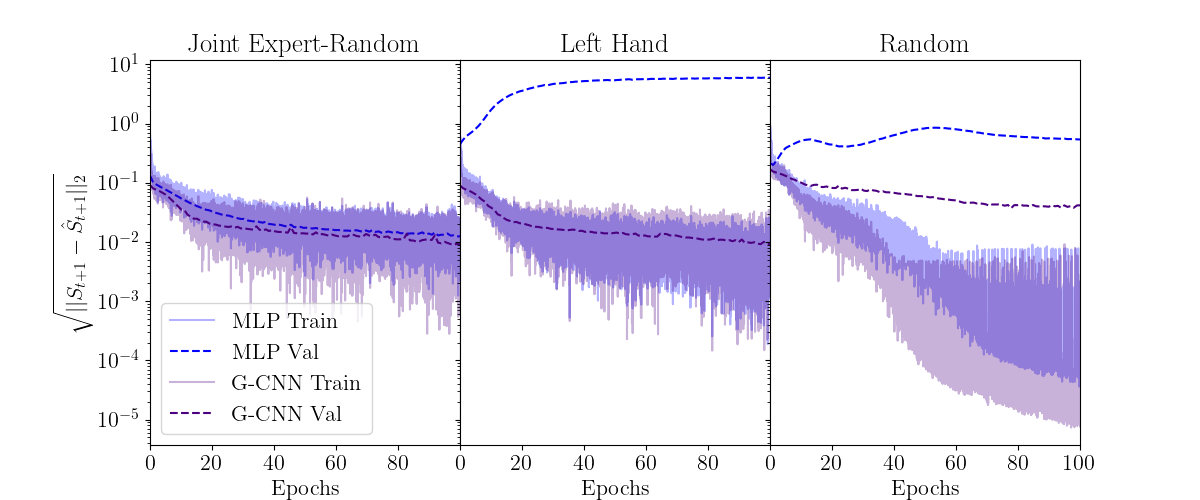
\includegraphics[width=.65\textwidth]{Figures/transition_model_loss.png}
	\caption{Transition Model RMS error, plotted against epochs for three different training
		datasets. Left, the joint expert-random dataset. Center, the same dataset as
		left, however, with only the left action taken. Right, solely transitions sampled
		from a random policy. These datasets contain 400,000 transitions. All plots have
		the same set of validation data with a 50/50 split of expert and random policy
		sampled data.}\label{fig:tm_cp}
\end{wrapfigure}

The training and validation loss for the three equivariant transition models (G-CNNs) are plotted against comparable multi layer perceptron (MLP) networks with the same depth and parameter count on these three different datasets. Each dataset contains $400,000$ transitions. In all three figures the model is validated on a new expert policy sampled dataset. This enables testing out of distribution generalisation.

In all cases the equivariant transition model outperforms the MLP. In the central plot of Figure~\ref{fig:tm_cp}, the equivariant model generalises to transitions that are out of the distribution of the ``Left Hand" training dataset. This is the key property of the equivariance exploiting the symmetry of the environment, such that if the state is transformed by a group action so is the policy.

Interestingly, the G-CNNs equivariance enables the model to generalise better than the MLP to the expert policy sampled validation set, when only trained on random policy data. This is notable because the steady state distributions of an expert and random policy are vastly different. Empirically, expert policies sample many more transitions at small angles, $|\theta| < 1^o$\footnote{See appendix Figure~\ref{fig:cp_hist}}. This is an encouraging result for learning the equivariant transition model online. The initial policy of an RL agent is often approximately random, and so the dataset for the transition model is mostly random. Our approach could deliver faster model learning in these early stages due its ability to generalise better to increasingly expert policies as the agent learns.

\begin{figure}
	\centering
	\begin{minipage}[b]{.5\textwidth}
		\centering
		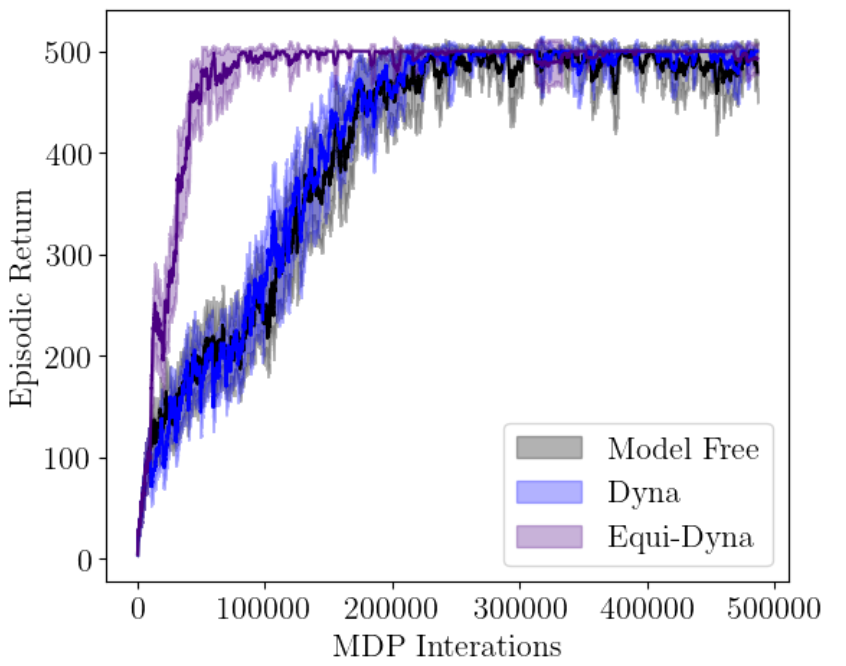
\includegraphics[width=\textwidth]{Figures/best_cp.png}
	\end{minipage}%
	\begin{minipage}[b]{.5\textwidth}
		\centering
		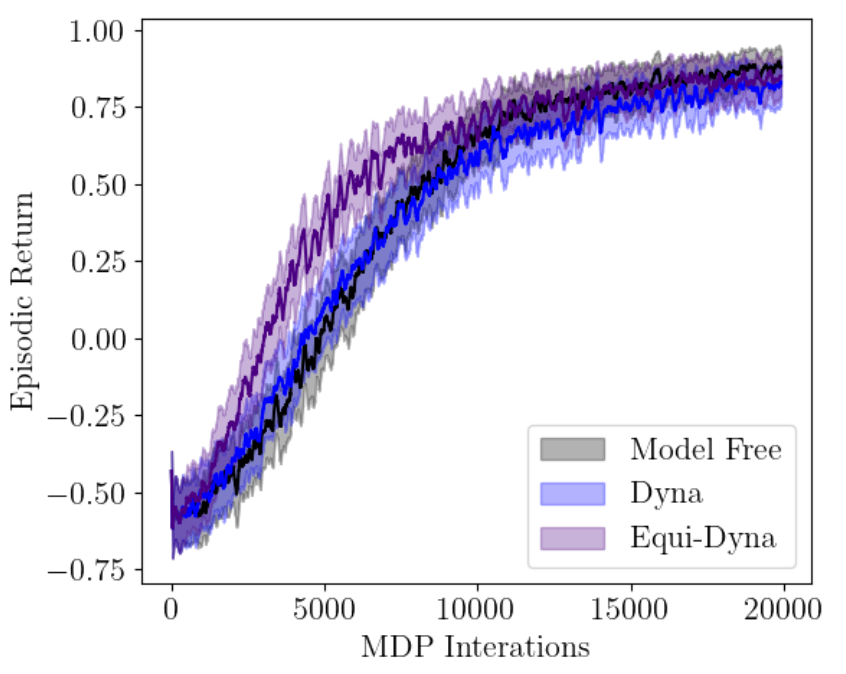
\includegraphics[width=\textwidth]{Figures/best_ctch.png}
	\end{minipage}%
	\caption{Left: Cart-Pole episodic return plotted against MDP interactions. Right: Catch episodic return plotted against MDP interactions. All agents were run across 128 random seeds with 2 standard errors plotted. The best planning ratios are plotted for all agents.}
	\label{fig:joint}
\end{figure}

\textbf{Planning Experiments.} The next set of experiments were performed with the models trained on joint expert-random datasets. A PPO two layer MLP agent samples experience from the real environment, and then from the pre-trained transition model. This is then iterated over 50 times. The ratio between the number of simulated transitions is the ``planning ratio". In Figure~\ref{fig:joint}, the planning ratios are eight and one for Equi-Dyna and Dyna, respectively. In the Catch environment both model based methods used a planning ratio of four. These values were found from a grid search across $[0.5, 1, 2, 4,  8]$.

From, both of the return curves in Figure~\ref{fig:joint} we see that the equivariant planning models do successfully improve the interaction efficiency of the agents. Further, they substantially improve upon the MLPs which are not equivariant. This confirms that the proximal pooling layer is an effective method to implement approximate equivariance in transition models.

\vspace{-10}
\section{Future Work}
The next steps are to focus on implementing online learning of transition models, and to implement further discrete symmetry groups. Additionally, an extension to Steerable-CNNs~\cite{weiler2019general} would extend the current method to continuous symmetry groups.

The other interesting avenue to pursue because of the G-CNN architecture is to leverage the ability to meta-learn the equivariant structure from experience using the method presented by~\cite{zhou2020meta}.

\newpage

\bibliography{equivariant_transition_models}
\newpage
\appendix
\section{Cart-Pole}
\begin{figure}[h]
	\centering
	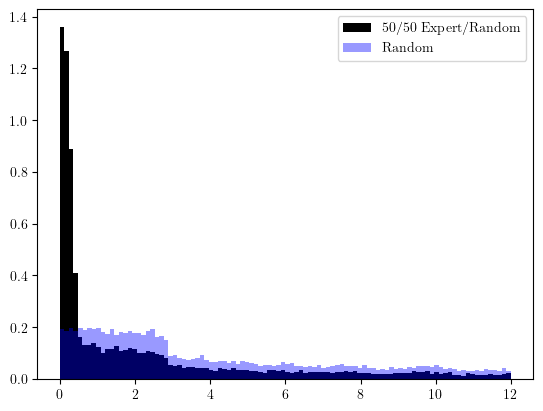
\includegraphics[width=0.7\textwidth]{Figures/angles_cp.png}
	\caption{Histogram of transitions by start angle in Cart-pole, sampled from the joint expert-random dataset and the random dataset}\label{fig:cp_hist}
\end{figure}



\end{document}

